\documentclass[border=3pt]{standalone}
\usepackage{amsmath}\usepackage{amssymb}
\usepackage{fontspec}\setsansfont{Arial}\renewcommand{\familydefault}{\sfdefault}
\usepackage{tikz}
\usetikzlibrary{arrows.meta,positioning,calc,fit,backgrounds,shapes.geometric}
\definecolor{titlegray}{HTML}{5F6B78}\definecolor{ent}{HTML}{7B8794}
\definecolor{fo}{HTML}{5AA9C4}\definecolor{ho}{HTML}{2E6B86}
\definecolor{inf}{HTML}{D98A3D}\definecolor{vio}{HTML}{9B86C4}
\definecolor{smac}{HTML}{2E8AA6}\definecolor{kgc}{HTML}{E7B15A}
\definecolor{fillteal}{HTML}{E3EEF2}\definecolor{fillamber}{HTML}{FBF0E2}
\definecolor{fillgrey}{HTML}{F1F3F5}\definecolor{fillviolet}{HTML}{EFEAF6}
\definecolor{inkmid}{HTML}{3D4751}\definecolor{distract}{HTML}{B3403A}
\begin{document}
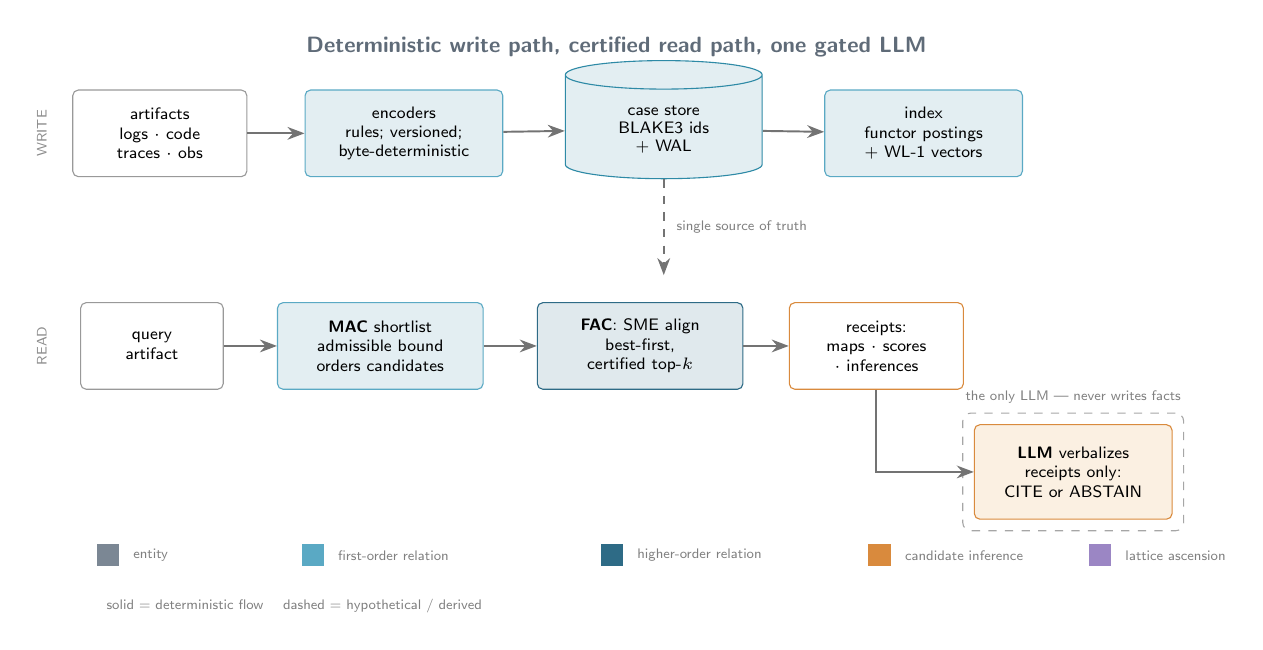
\begin{tikzpicture}[
  font=\sffamily,>=Stealth,
  ttl/.style={font=\sffamily\fontsize{8}{9}\selectfont\bfseries, color=titlegray, align=center},
  sub/.style={font=\sffamily\fontsize{6}{7}\selectfont, color=black!55, align=center},
  micro/.style={font=\sffamily\fontsize{5.2}{6}\selectfont, color=black!50, align=center},
  enode/.style={circle, draw=ent, fill=ent, text=white, font=\sffamily\fontsize{5.2}{6}\selectfont, inner sep=0pt, minimum size=6.5mm, align=center},
  fnode/.style={circle, draw=fo, fill=fo, text=white, font=\sffamily\fontsize{5.2}{6}\selectfont, inner sep=0pt, minimum size=7mm, align=center},
  hnode/.style={circle, draw=ho, fill=ho, text=white, font=\sffamily\fontsize{5.2}{6}\selectfont, inner sep=0pt, minimum size=7.5mm, align=center},
  pbox/.style={rounded corners=2pt, draw, align=center, inner sep=3pt, font=\sffamily\fontsize{6}{7}\selectfont},
  flowarr/.style={->, line width=0.7pt, color=black!55},
  horel/.style={->, line width=0.7pt, color=ho},
  forel/.style={->, line width=0.6pt, color=fo!80},
]

\node[ttl] at (7,5.5) {Deterministic write path, certified read path, one gated LLM};
% write lane
\node[micro,rotate=90,color=black!45] at (-0.3,4.4) {WRITE};
\node[pbox,draw=black!40,fill=white,text width=2.0cm,minimum height=1.1cm] (art) at (1.2,4.4) {artifacts\\logs $\cdot$ code\\traces $\cdot$ obs};
\node[pbox,draw=fo,fill=fillteal,text width=2.3cm,minimum height=1.1cm] (enc) at (4.3,4.4) {encoders\\rules; versioned;\\byte-deterministic};
\node[cylinder,shape border rotate=90,draw=smac,fill=fillteal,aspect=0.28,minimum width=2.5cm,minimum height=1.5cm,inner sep=2pt,font=\sffamily\fontsize{5.6}{6.4}\selectfont,align=center] (store) at (7.6,4.45) {case store\\BLAKE3 ids\\+ WAL};
\node[pbox,draw=fo,fill=fillteal,text width=2.3cm,minimum height=1.1cm] (idx) at (10.9,4.4) {index\\functor postings\\+ WL-1 vectors};
\draw[flowarr] (art)--(enc); \draw[flowarr] (enc)--(store); \draw[flowarr] (store)--(idx);
% read lane
\node[micro,rotate=90,color=black!45] at (-0.3,1.7) {READ};
\node[pbox,draw=black!40,fill=white,text width=1.6cm,minimum height=1.1cm] (q) at (1.1,1.7) {query\\artifact};
\node[pbox,draw=fo,fill=fillteal,text width=2.4cm,minimum height=1.1cm] (mac) at (4.0,1.7) {\textbf{MAC} shortlist\\admissible bound\\orders candidates};
\node[pbox,draw=ho,fill=ho!15,text width=2.4cm,minimum height=1.1cm] (fac) at (7.3,1.7) {\textbf{FAC}: SME align\\best-first,\\certified top-$k$};
\node[pbox,draw=inf,fill=white,text width=2.0cm,minimum height=1.1cm] (rec) at (10.3,1.7) {receipts:\\maps $\cdot$ scores\\$\cdot$ inferences};
\draw[flowarr] (q)--(mac); \draw[flowarr] (mac)--(fac); \draw[flowarr] (fac)--(rec);
\draw[flowarr,dashed] (store)-- node[micro,right=1pt]{single source of truth} (7.6,2.6);
\node[pbox,draw=inf,fill=fillamber,text width=2.3cm,minimum height=1.2cm] (llm) at (12.8,0.1) {\textbf{LLM} verbalizes\\receipts only:\\CITE or ABSTAIN};
\node[draw=black!35,dashed,rounded corners=3pt,fit=(llm),inner sep=4pt,label={[micro]above:the only LLM --- never writes facts}] {};
\draw[flowarr] (rec)|-(llm);
% legend
\foreach \x/\c/\t in {0.4/ent/entity,3.0/fo/{first-order relation},6.8/ho/{higher-order relation},10.2/inf/{candidate inference},13.0/vio/{lattice ascension}}
 {\fill[\c] (\x,-1.1) rectangle ++(0.28,0.28); \node[micro,anchor=west] at (\x+0.34,-0.96) {\t};}
\node[micro,anchor=west] at (0.4,-1.6) {solid = deterministic flow \quad dashed = hypothetical / derived};

\end{tikzpicture}
\end{document}
